\section{Numerical Results}
\label{sec:results}

For our experiments we have used RMACC Summit Supercomputer in University of Colorado, Boulder (through XSEDE). Each node has 24 cores and it uses Intel Xeon E5-2680 with $4.84GB$ of memory per core.

For these experiments for \mm~ we have multiplied a banded matrix with itself, assuming that the matrix is being multiplied with a separate matrix, so not using any information from the left-hand side matrix for the right-hand side one.

Figure\ref{fig:weak1} shows the weak scaling for two banded matrices.

\begin{figure}[tbh]
 \centering
 \Description{Description}
 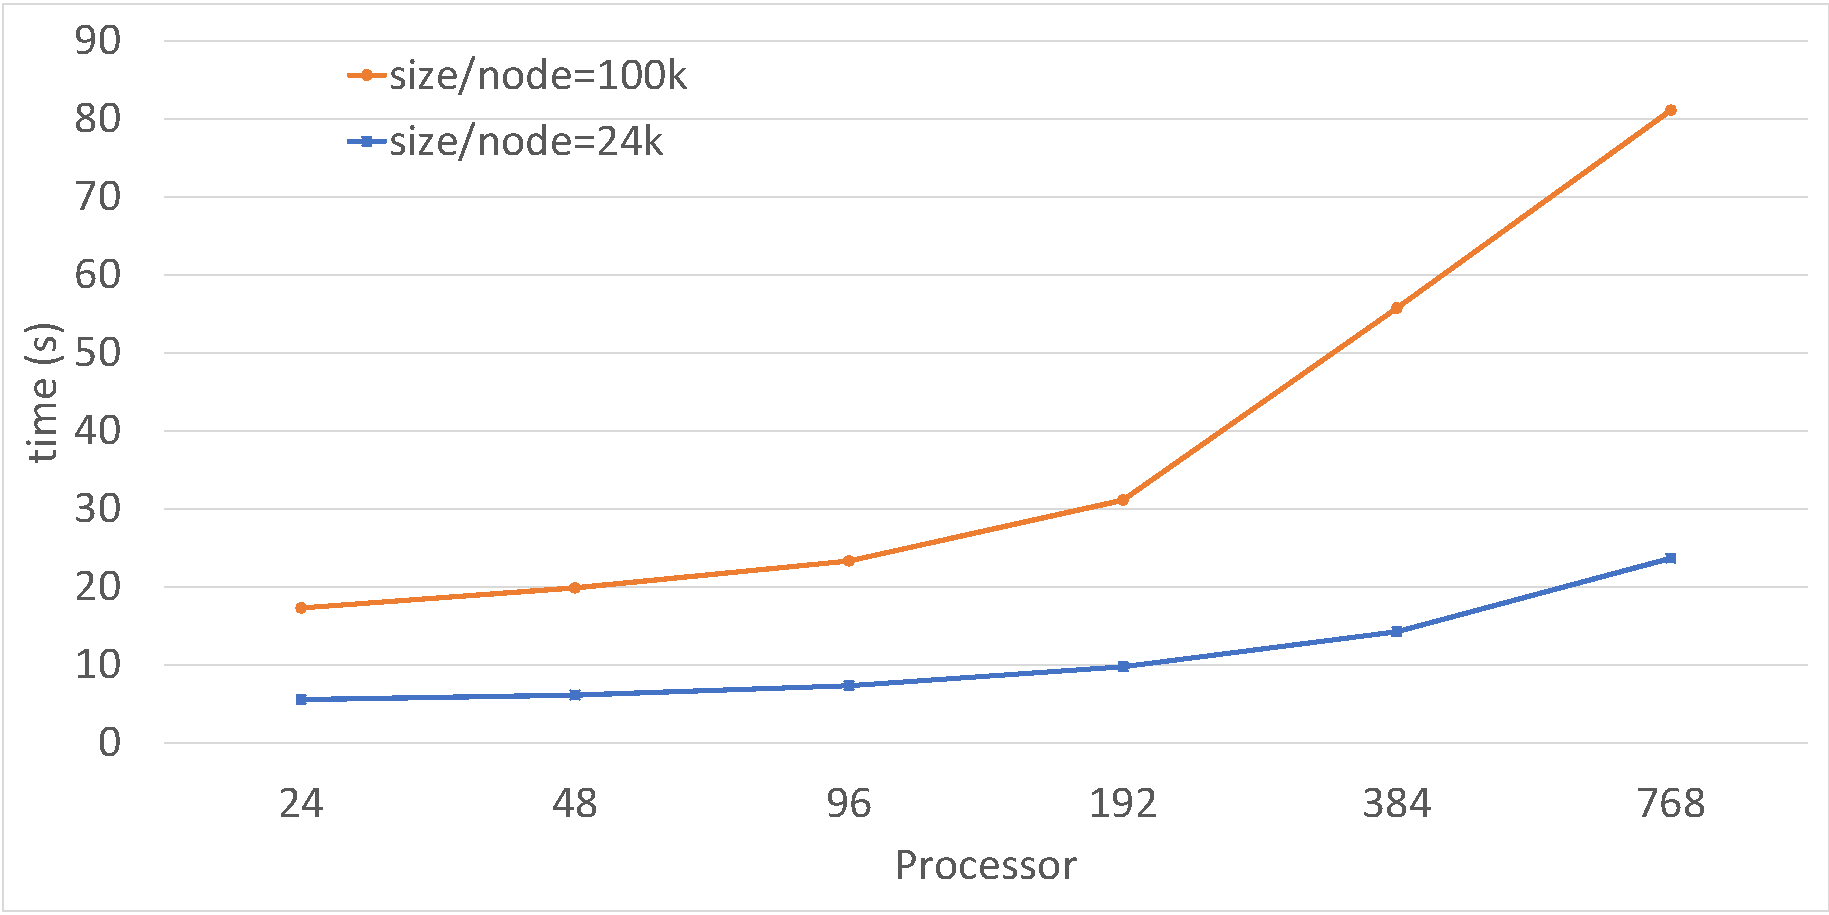
\includegraphics[width=8.5cm,height=4.8cm]{./figures/weak1.pdf}
 \caption{Weak scaling for two banded matrices}
 \label{fig:weak1}
\end{figure}

Figure\ref{fig:strong1} is the strong scaling for five banded matrices of the same size (192k), but with different bandwidth. The legend shows the density ($\frac{nonzero}{size^2}$) of each matrix.

\begin{figure}[tbh]
 \centering
 \Description{Description}
 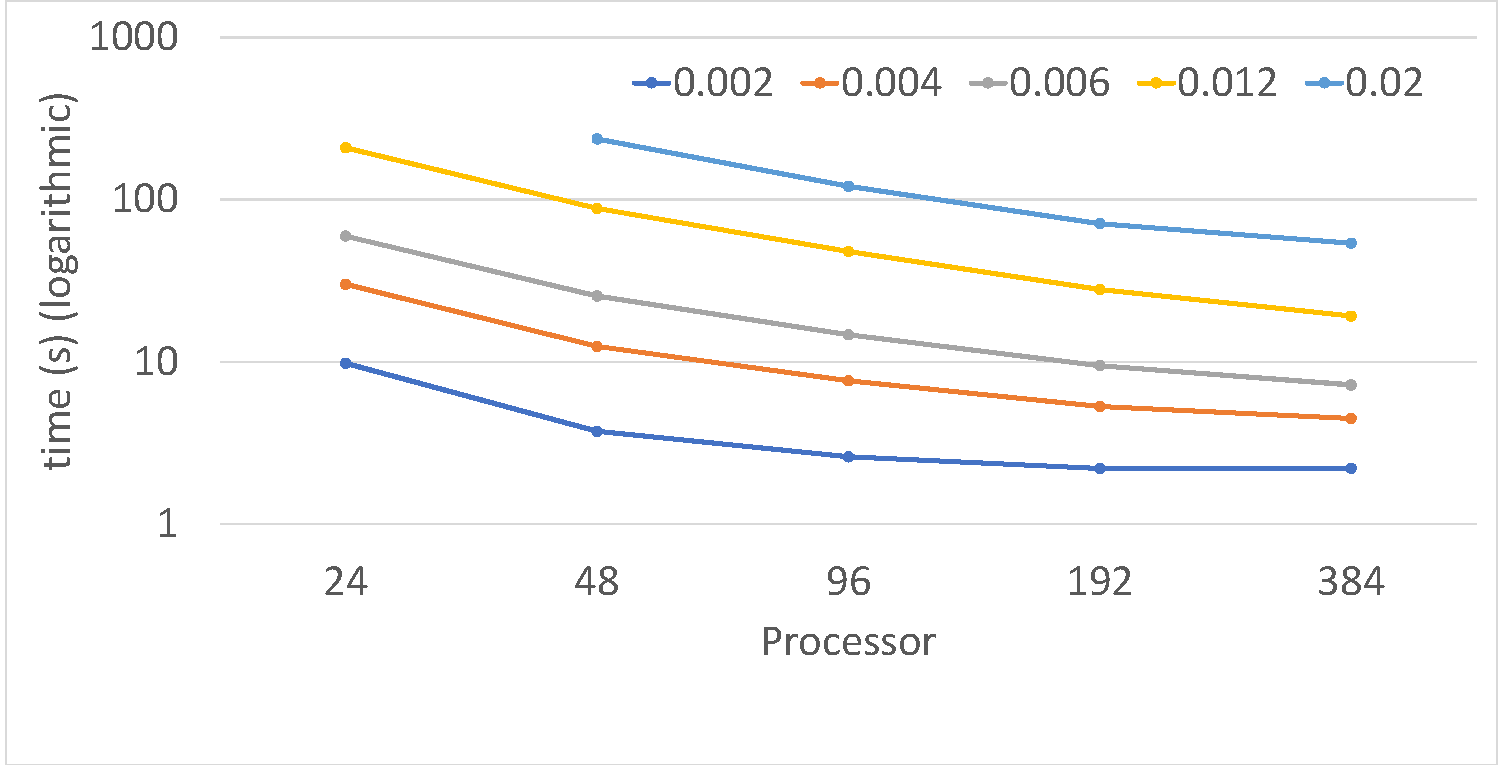
\includegraphics[width=8.5cm,height=4.9cm]{./figures/strong1.pdf}
 \caption{Strong scaling for five banded matrices of the same size (192k), but with different bandwidth}
 \label{fig:strong1}
\end{figure}

Figure\ref{fig:petsc1} compares the strong scaling between our solver and PETSc. For the matrices with lower density (more sparse) PETSc performs better when using higher number of processes, but for denser matrices our solver is faster. In multigrid hierarchy, the coarse matrices get denser as we go to lower levels, so it becomes expensive to perform \mm~ and having a fast matrix-matrix product would improve the setup cost significantly.

\begin{figure}[tbh]
 \centering
 \Description{Description}
 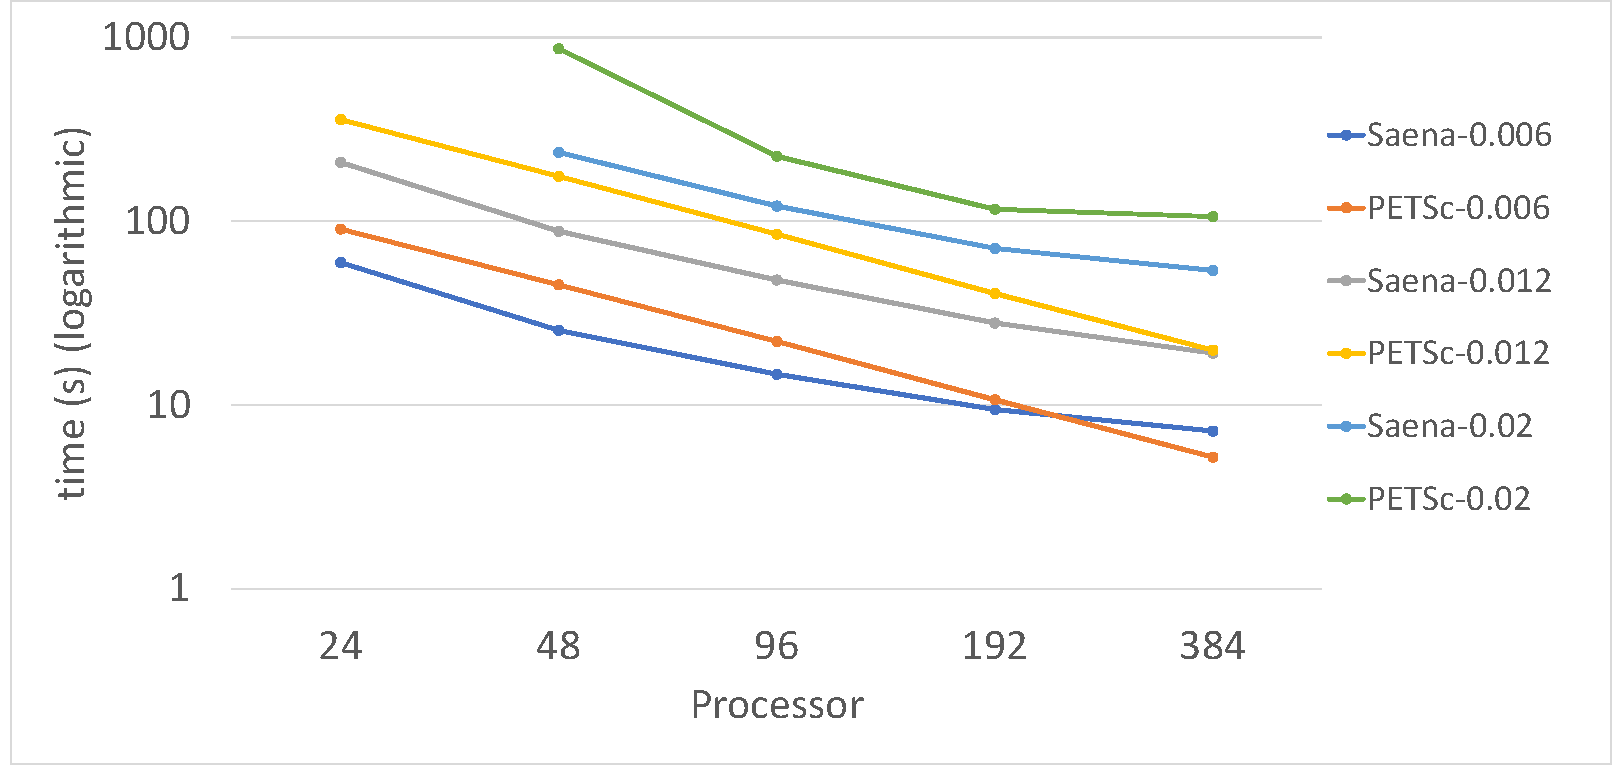
\includegraphics[width=8.5cm,height=4.4cm]{./figures/petsc1.pdf}
 \caption{Comparison of the the strong scaling between our solver and PETSc. The number for each line shows the density for that matrix.}
 \label{fig:petsc1}
\end{figure}

